\documentclass[12pt,spanish]{article}
\usepackage[spanish]{babel}
\usepackage{graphicx}
\usepackage{multirow}
\usepackage{float}
\usepackage{enumitem}
\usepackage[hidelinks]{hyperref}
\usepackage{array}
\graphicspath{ {/home/csp98/latex/img/} {../diagramas/} {./img/} {../../LaTeX/img/}}
\selectlanguage{spanish}
\usepackage[utf8]{inputenc}
\usepackage{graphicx}
\usepackage[a4paper,left=3cm,right=2cm,top=2.5cm,bottom=2.5cm]{geometry}
\makeindex

\begin{document}
\begin{titlepage}

\newlength{\centeroffset}
\setlength{\centeroffset}{-0.5\oddsidemargin}
\addtolength{\centeroffset}{0.5\evensidemargin}
\thispagestyle{empty}

\noindent\hspace*{\centeroffset}\begin{minipage}{\textwidth}

\centering

\includegraphics[width=0.9\textwidth]{logo_ugr.jpg}\\[1.4cm]

\textsc{ \Large Fundamentos de Ingeniería del Software\\[0.2cm]}
\textsc{GRADO EN INGENIERÍA INFORMÁTICA}\\[1cm]

{\Huge\bfseries Práctica 2. Modelos de casos de uso\\
}
\noindent\rule[-1ex]{\textwidth}{3pt}\\[3.5ex]
{\large\bfseries Primera parte}
\end{minipage}

\vspace{2.5cm}
\noindent\hspace*{\centeroffset}
\begin{minipage}{\textwidth}
\centering

\textbf{Autores}\\ {José Baena Cobos \\ José Miguel Pelegrina Pelegrina\\Carlos Sánchez Páez}\\[2.5ex]

\includegraphics[width=0.3\textwidth]{etsiit_logo.png}\\[0.1cm]
\vspace{1.5cm}

\includegraphics[width=0.2\textwidth]{lsi.png}\\[0.1cm]
\vspace{1cm}
\textsc{Escuela Técnica Superior de Ingenierías Informática y de Telecomunicación}\\
\vspace{1cm}
\textsc{Curso 2017-2018}
\end{minipage}
\end{titlepage}
\tableofcontents
\thispagestyle{empty}
\listoffigures
\listoftables
\newpage
\setcounter{page}{1}
%%%%%%%%%%%%%%%%%%%%%%%%Comienzo del documento%%%%%%%%%%%%%%%%%%%%%%%%%%%%%%%

\section{Diagramas de casos de uso}

\subsection{Identificación de actores}
Los actores que participarán en esta práctica son los siguientes:
\begin{itemize}
\item Emisor.
\item Socio.
\item Receptor.
\item Empleado de almacén.
\item Encargado de oficina.
\item Conductor.
\end{itemize}
\subsection{Identificación de casos de uso}
Los supuestos de casos de uso son:
\begin{enumerate}[label=\textbf{CU-\arabic*}]
	\item Enviar un paquete.
	\begin{enumerate}[label=\textbf{CU-1.\arabic*}]
		\item Identificación en el sistema.
		\item Seleccionar tarifa.
		\item Elegir franja horaria de entrega.
		\item Concertar recogida.
	\end{enumerate}
	\item Consultar información sobre el paquete en tránsito.
	\begin{enumerate}[label=\textbf{CU-2.\arabic*}]
		\item Identificación en el sistema.
		\item Resolver incidencias.
		\item Consultar fecha de entrega.
		\item Consultar localización actual.
	\end{enumerate}
	\item Trazar la ruta que realizará cada vehículo de la flota.
	\begin{enumerate}[label=\textbf{CU-3.\arabic*}]
		\item Consulta de paquetes a entregar o recoger.
		\item Consulta del destino de los paquetes.	
	\end{enumerate}
	\item Dirigir a los empleados.
	\begin{enumerate}[label=\textbf{CU-4.\arabic*}]
		\item Asignar conductores a la flota.
		\item Asignar trabajo a los empleados de almacén.	
	\end{enumerate}
	\item Valorar el servicio ofrecido.
	\begin{enumerate}[label=\textbf{CU-5.\arabic*}]
		\item Identificación en el sistema.
		\item Puntuación del envío.
		\item Resolución de posibles incidencias.
	\end{enumerate}
	\item Gestionar los socios.
	\begin{enumerate}[label=\textbf{CU-6.\arabic*}]
		\item Alta.
		\item Baja.
		\item Modificación de datos.
		\item Consulta de datos.
	\end{enumerate}

\end{enumerate}

\begin{figure}[H]
\centering
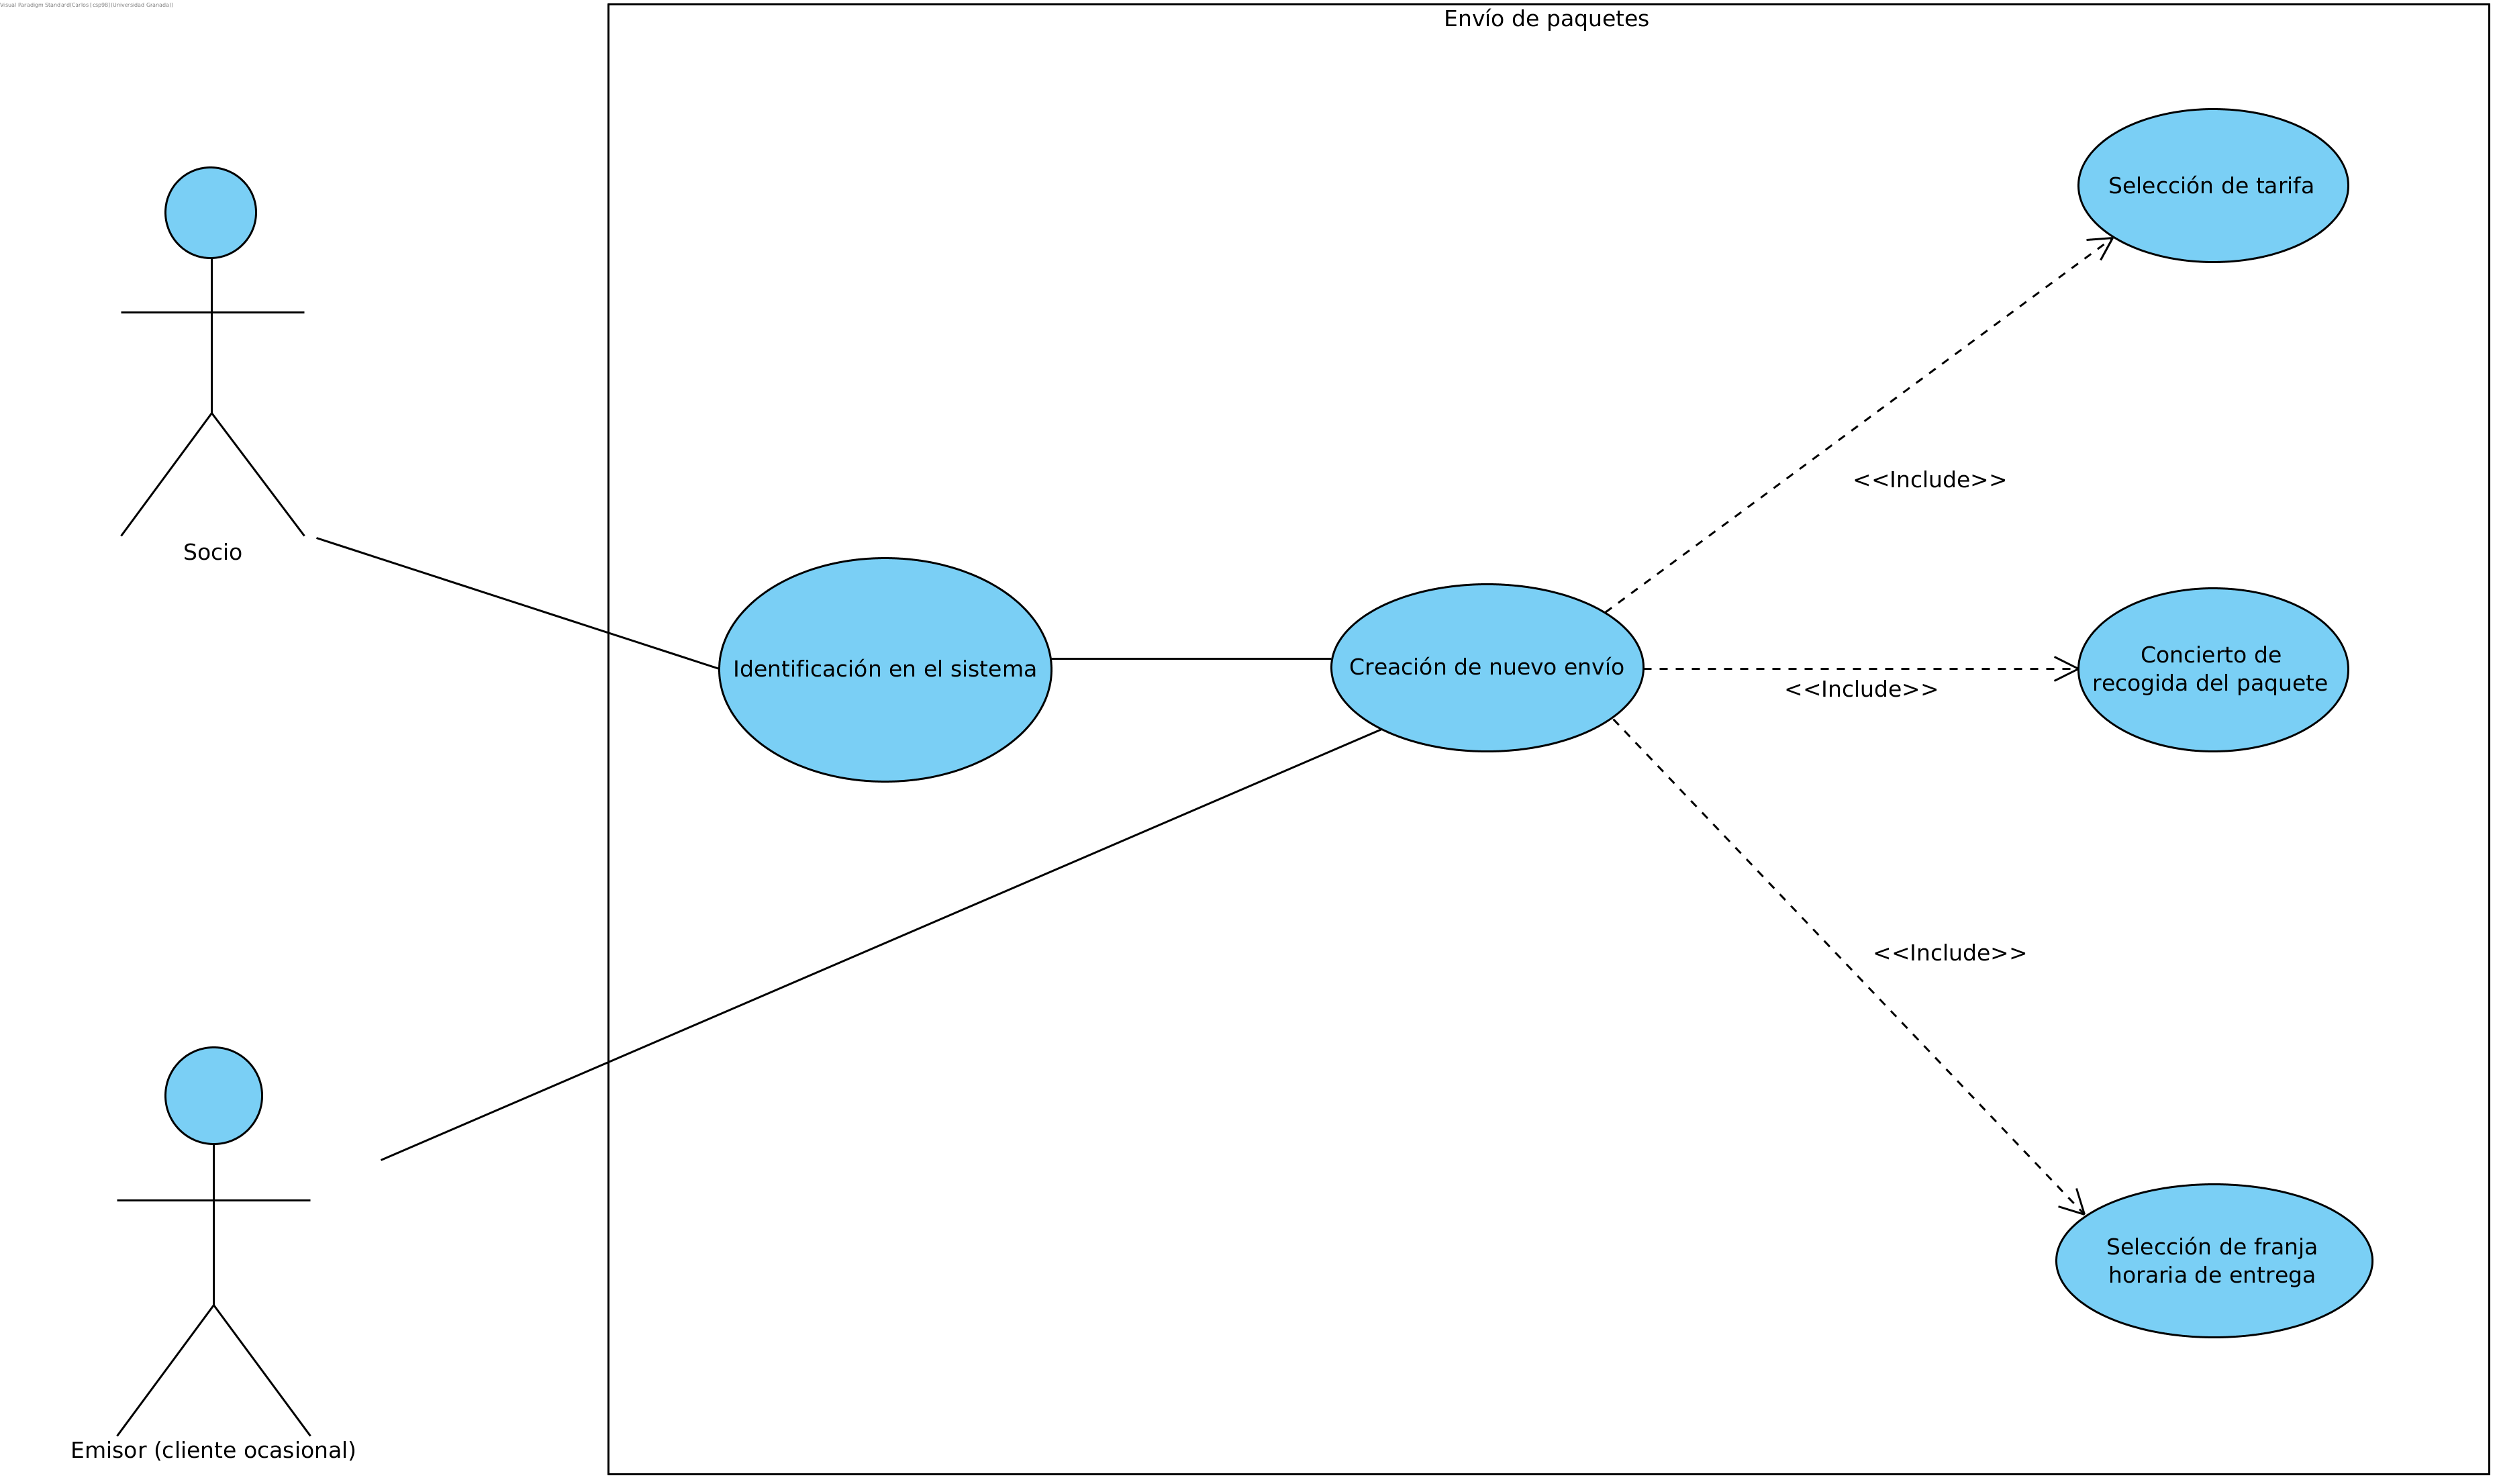
\includegraphics[scale=0.5]{enviar_paquete.png}
\caption{Enviar paquete}
\end{figure}

\begin{figure}[H]
\centering
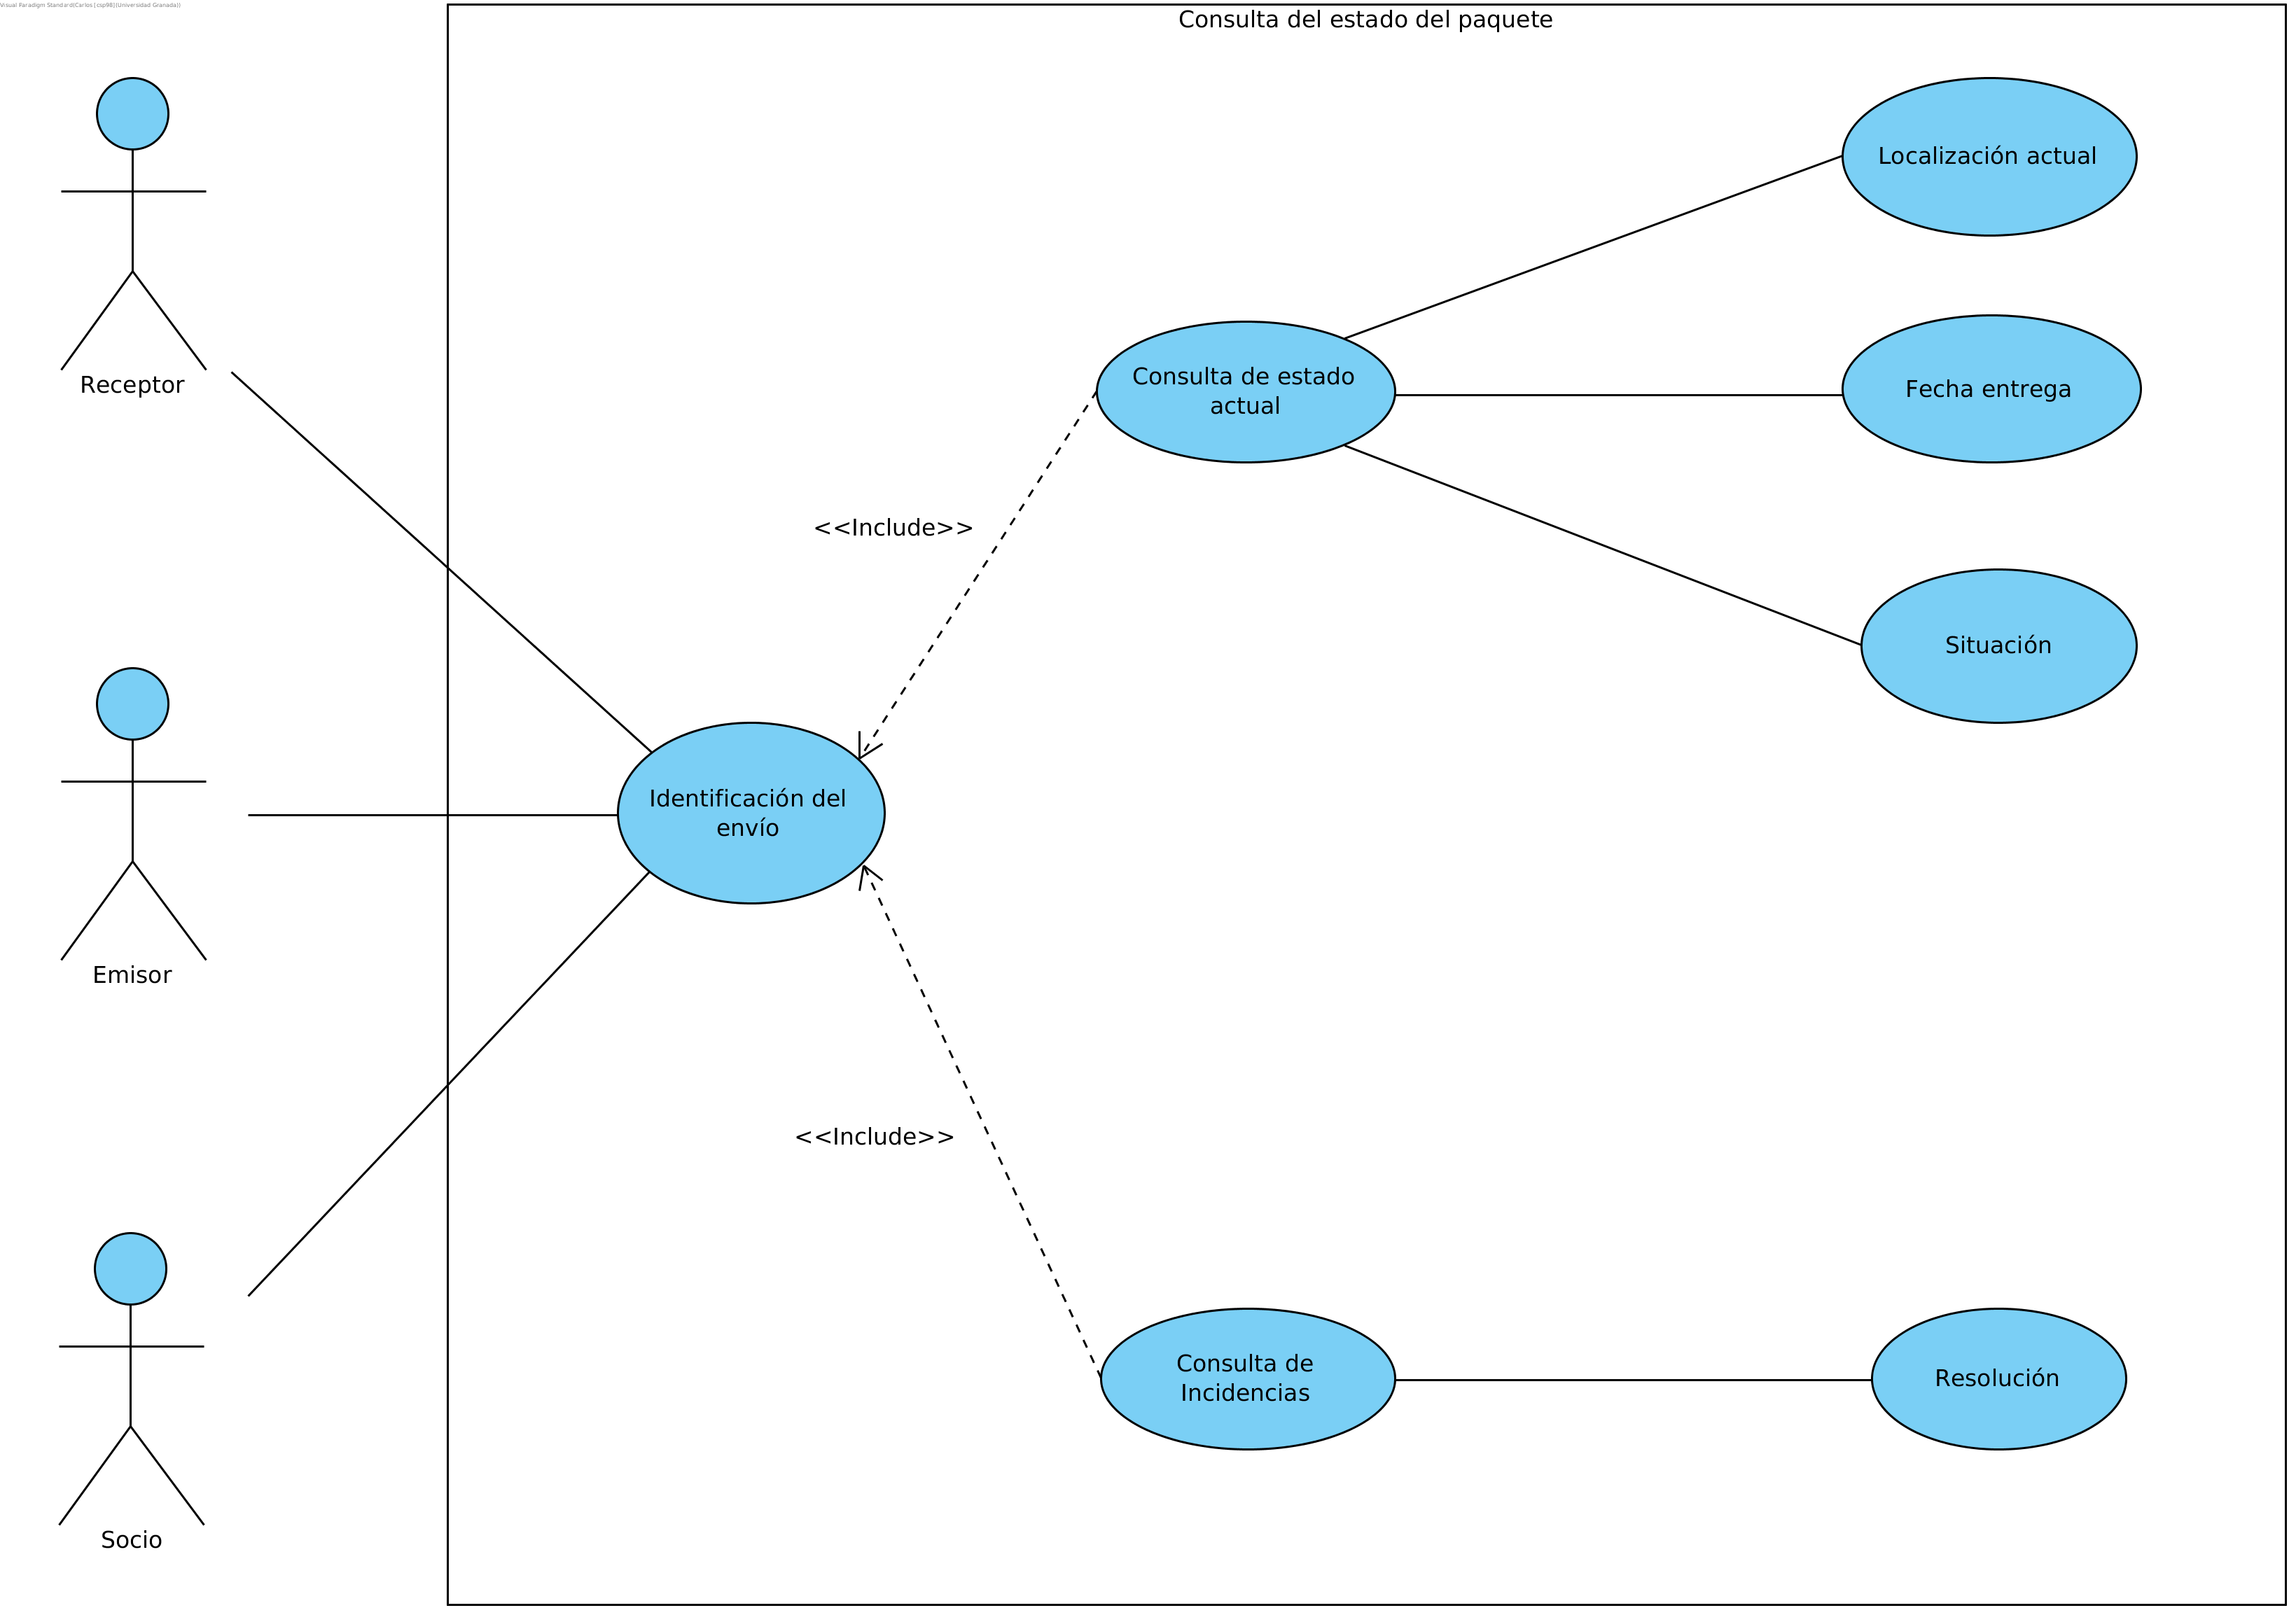
\includegraphics[scale=0.5]{consultar_estado.png}
\caption{Consultar estado del paquete}
\end{figure}

\begin{figure}[H]
\centering
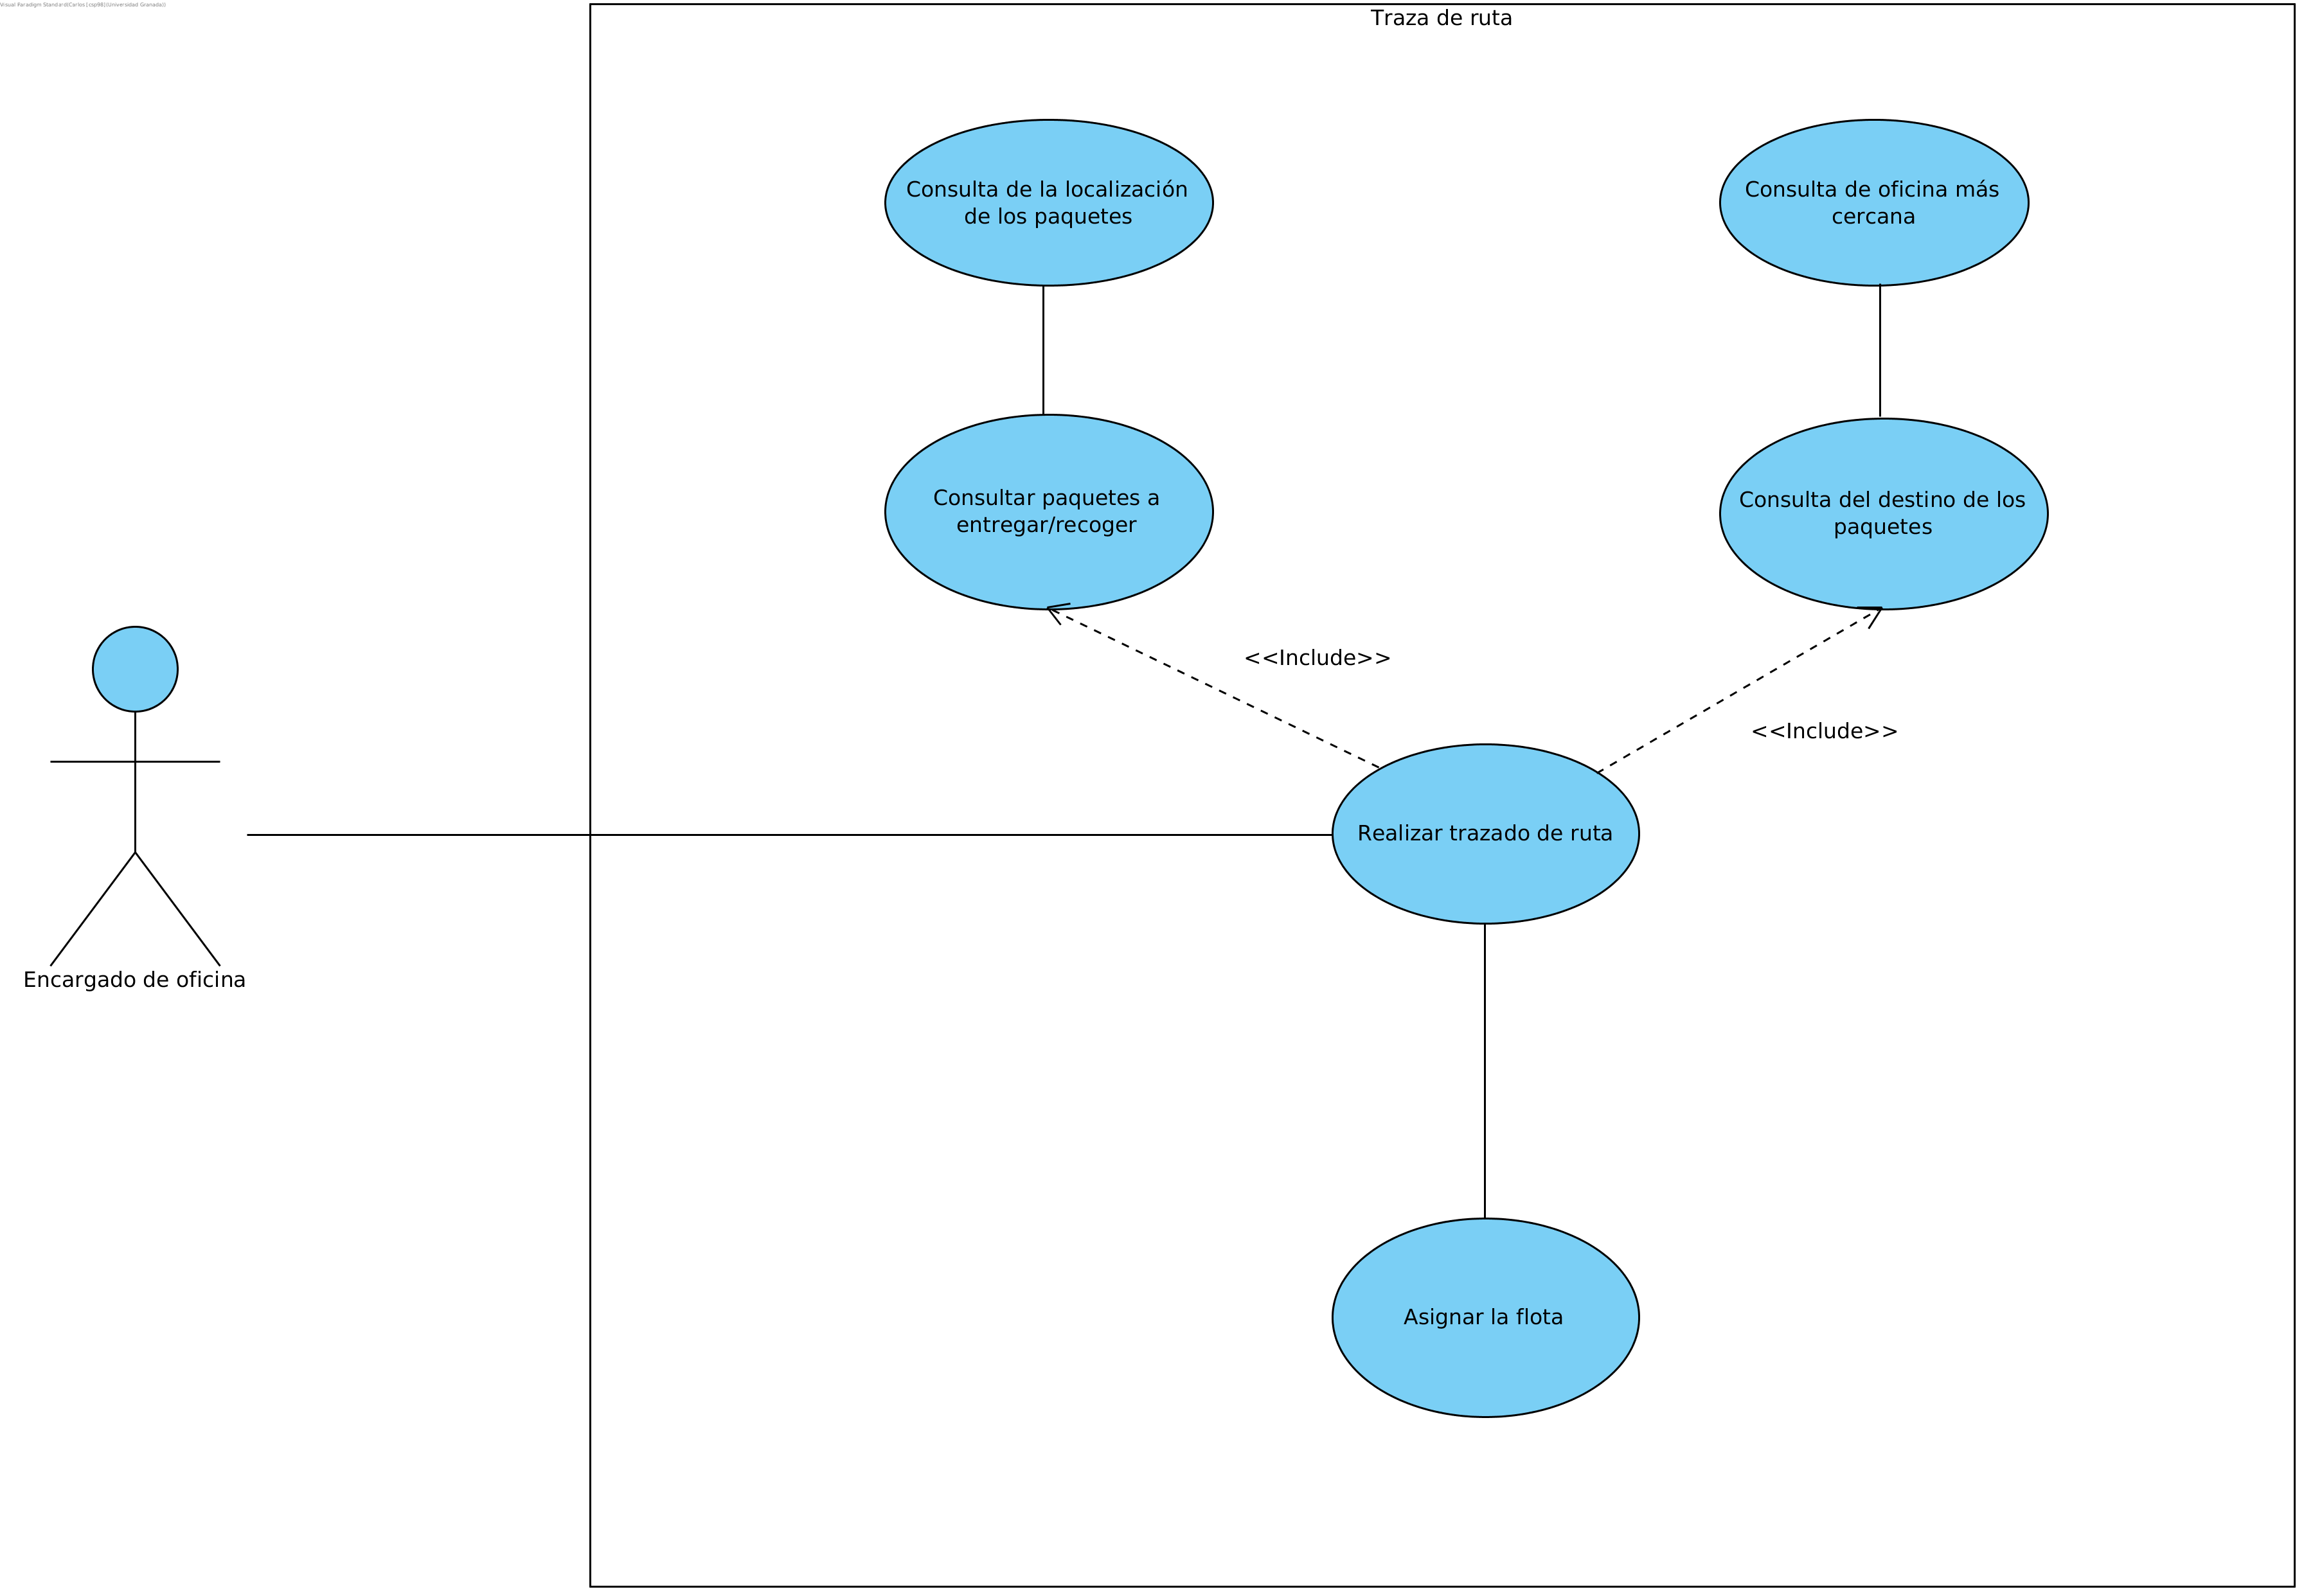
\includegraphics[scale=0.5]{trazar_ruta.png}
\caption{Trazar la ruta}
\end{figure}


\begin{figure}[H]
\centering
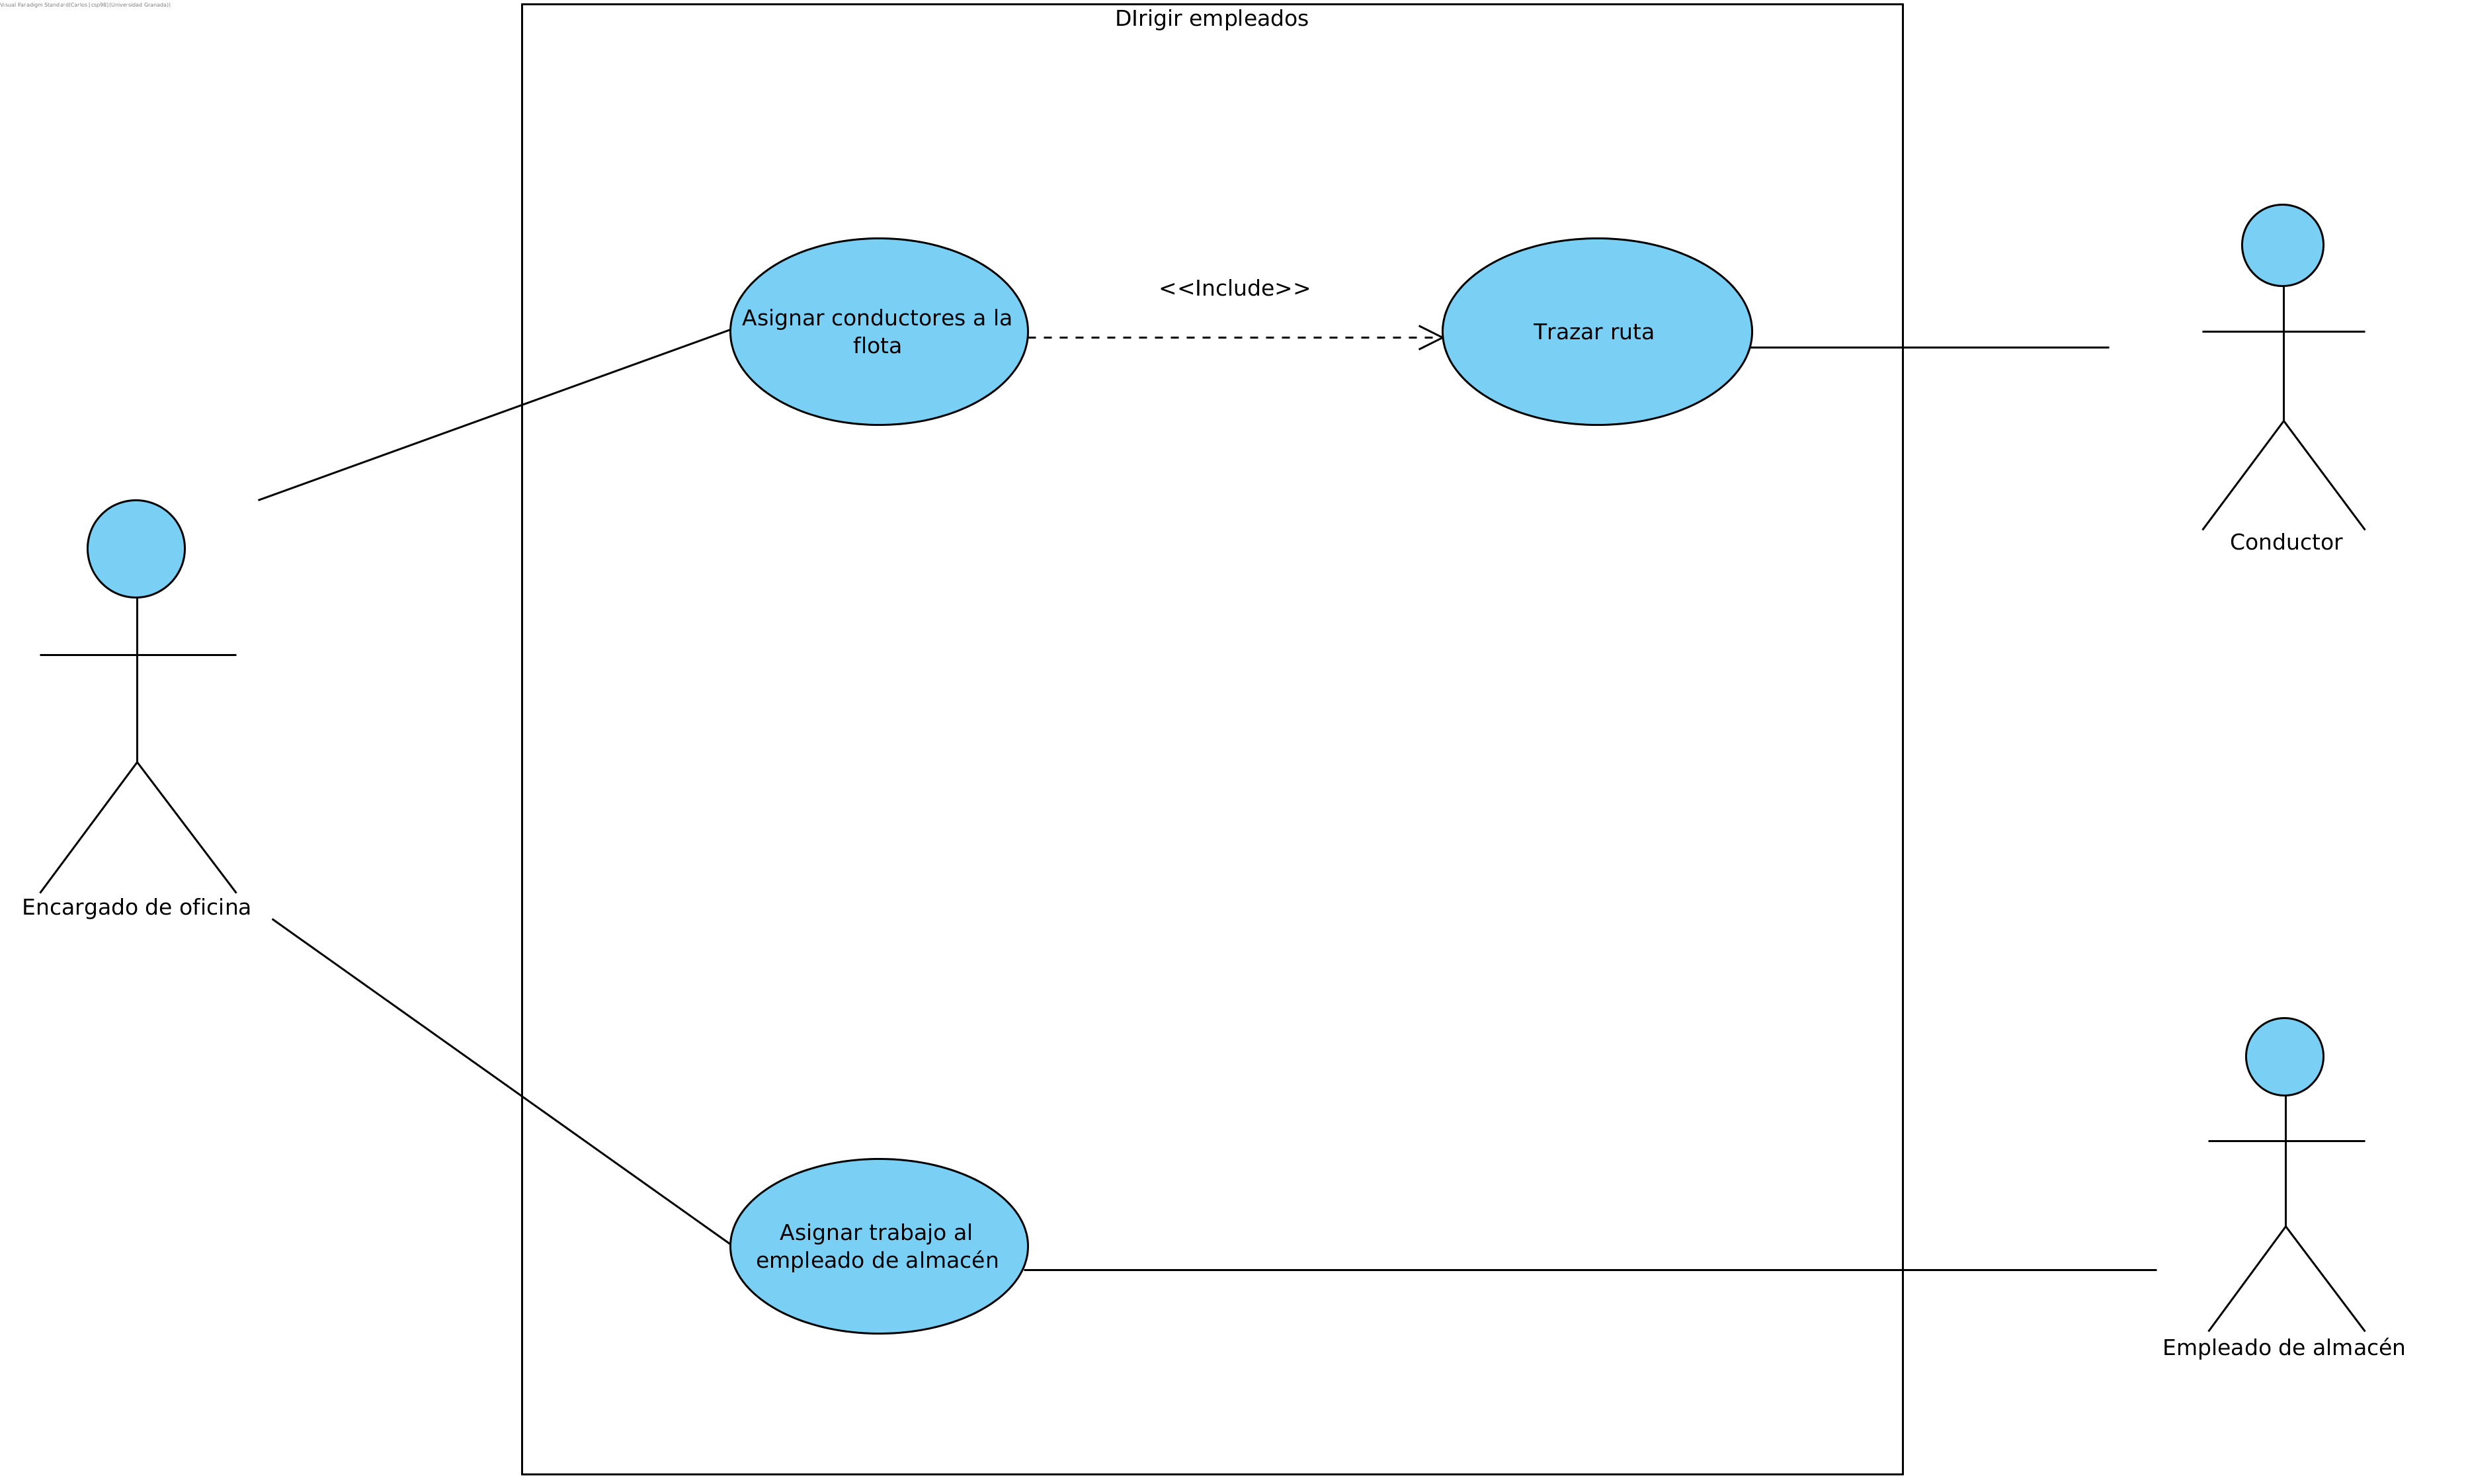
\includegraphics[scale=0.5]{dirigir_empleados.png}
\caption{Dirigir a los empleados}
\end{figure}


\begin{figure}[H]
\centering
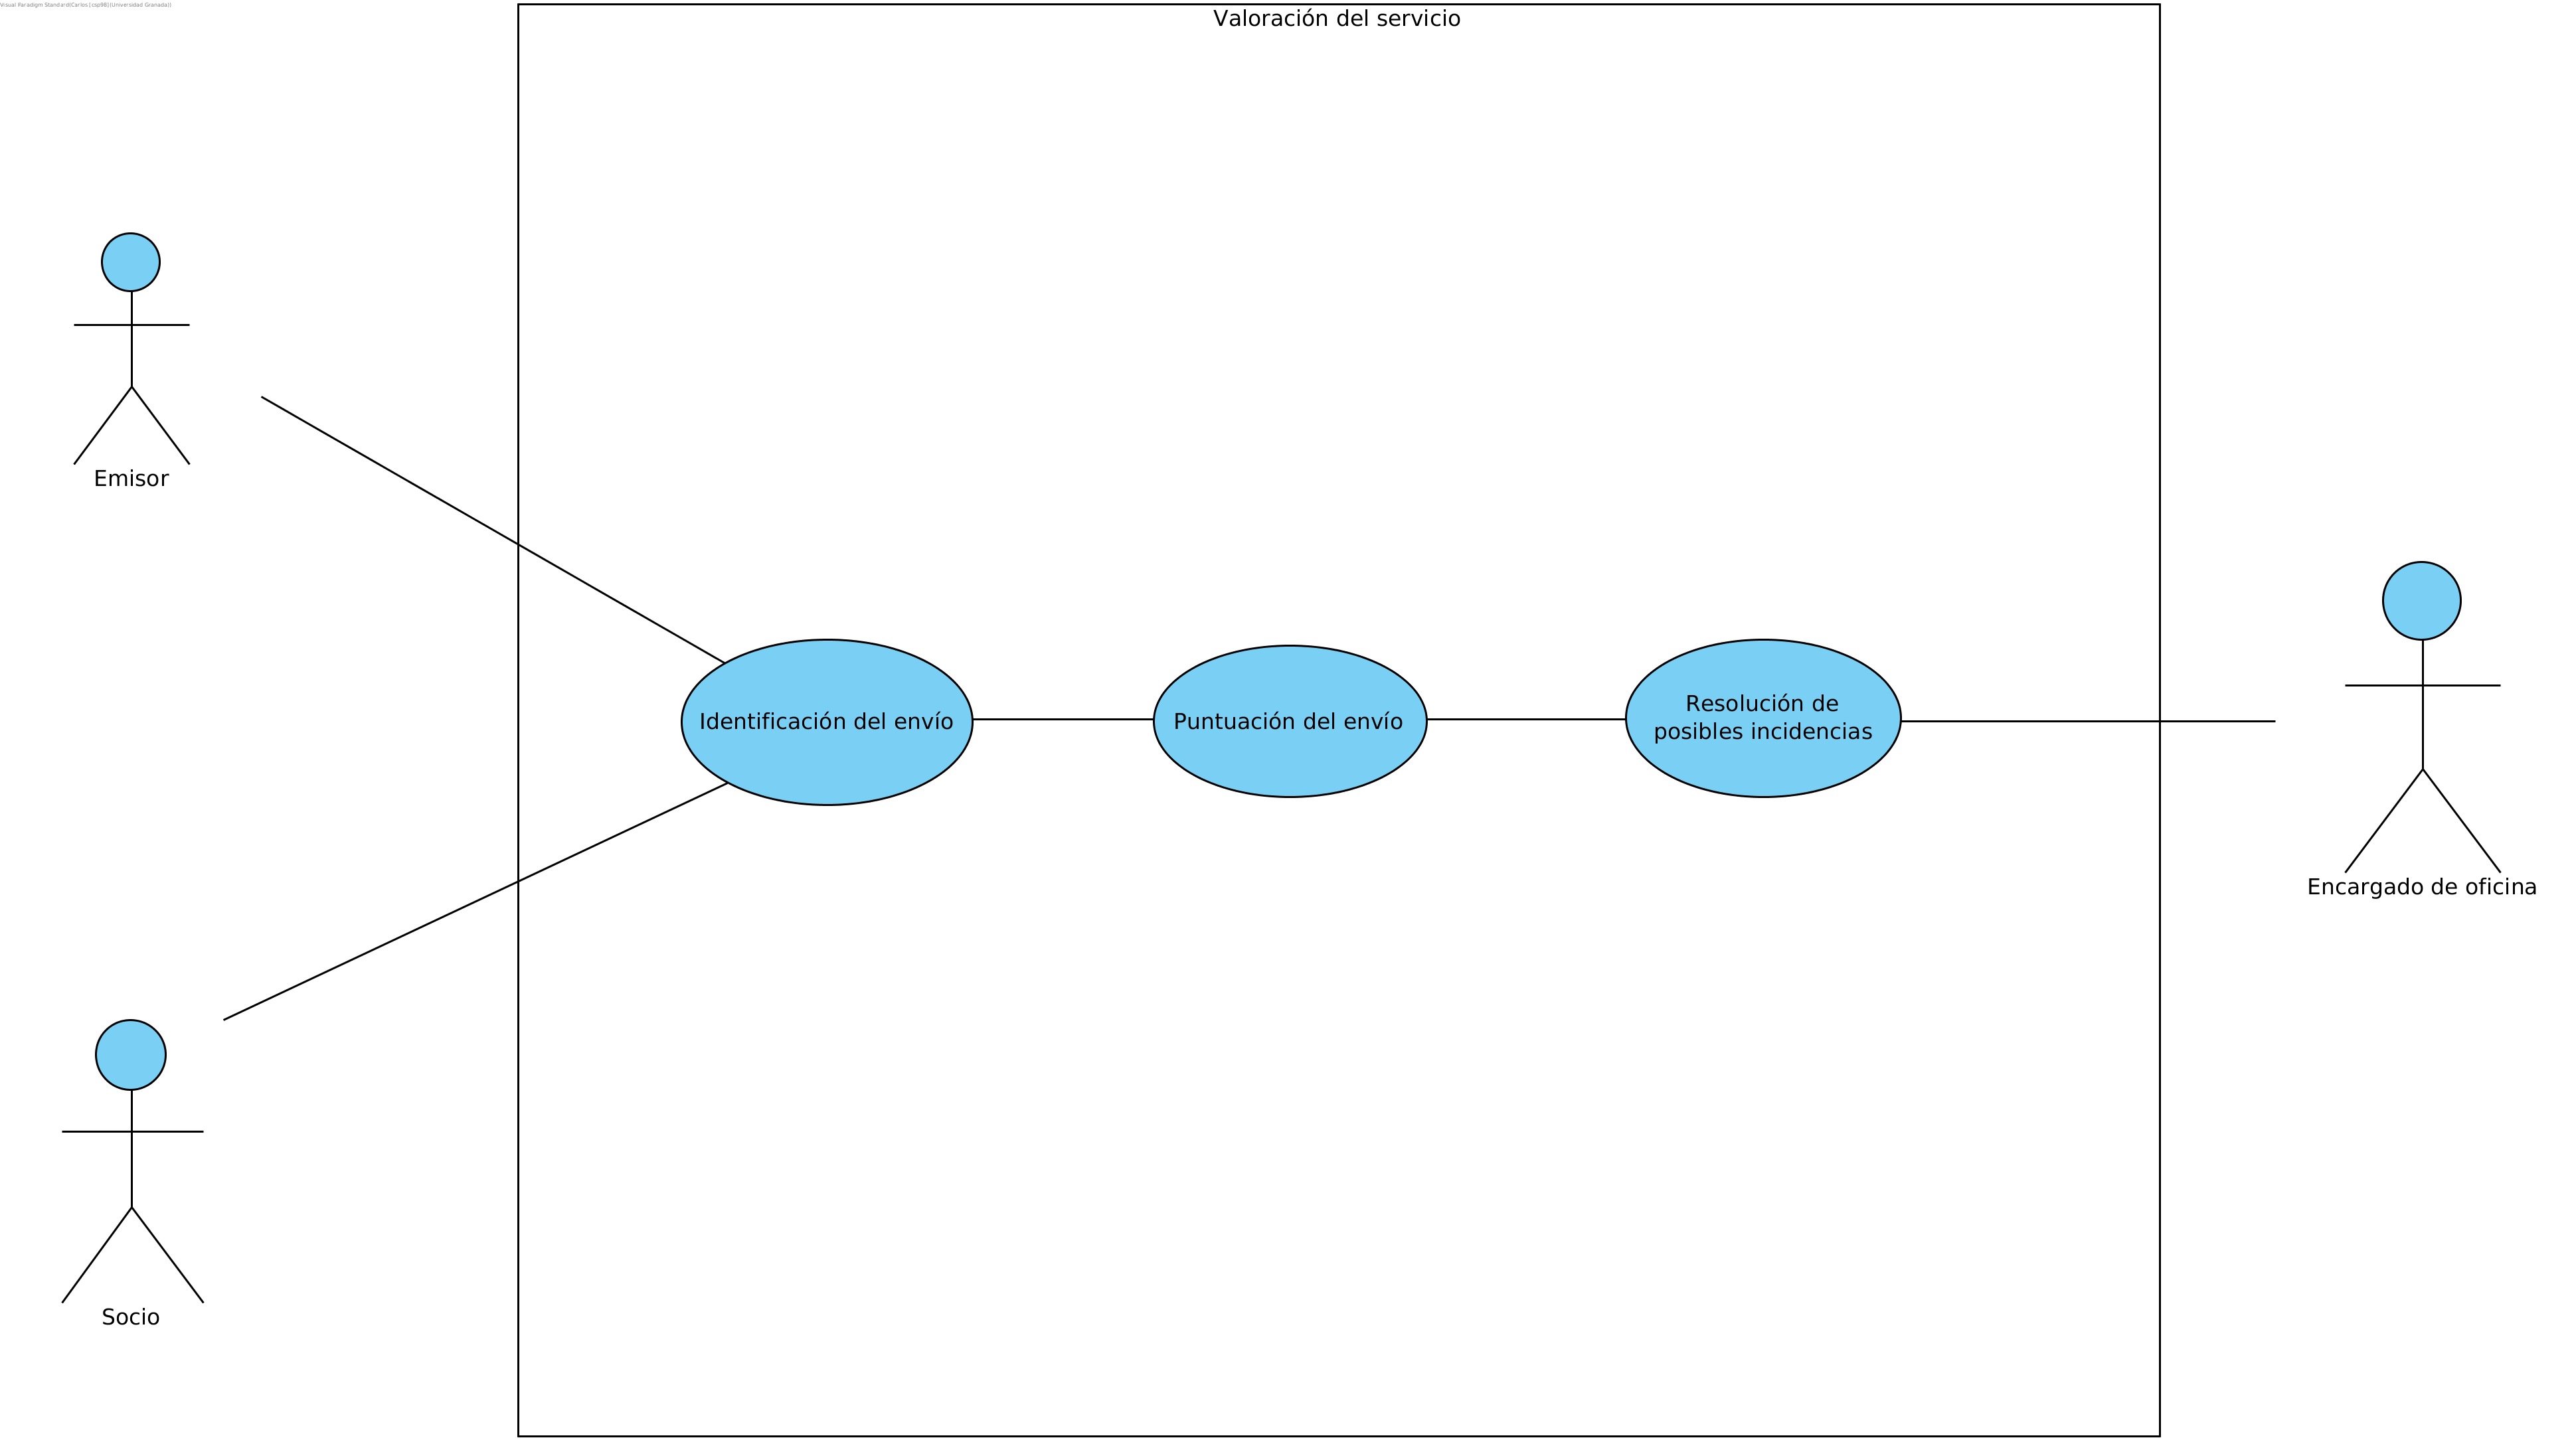
\includegraphics[scale=0.5]{valorar_servicio.png}
\caption{Valorar el servicio}
\end{figure}

\begin{figure}[H]
\centering
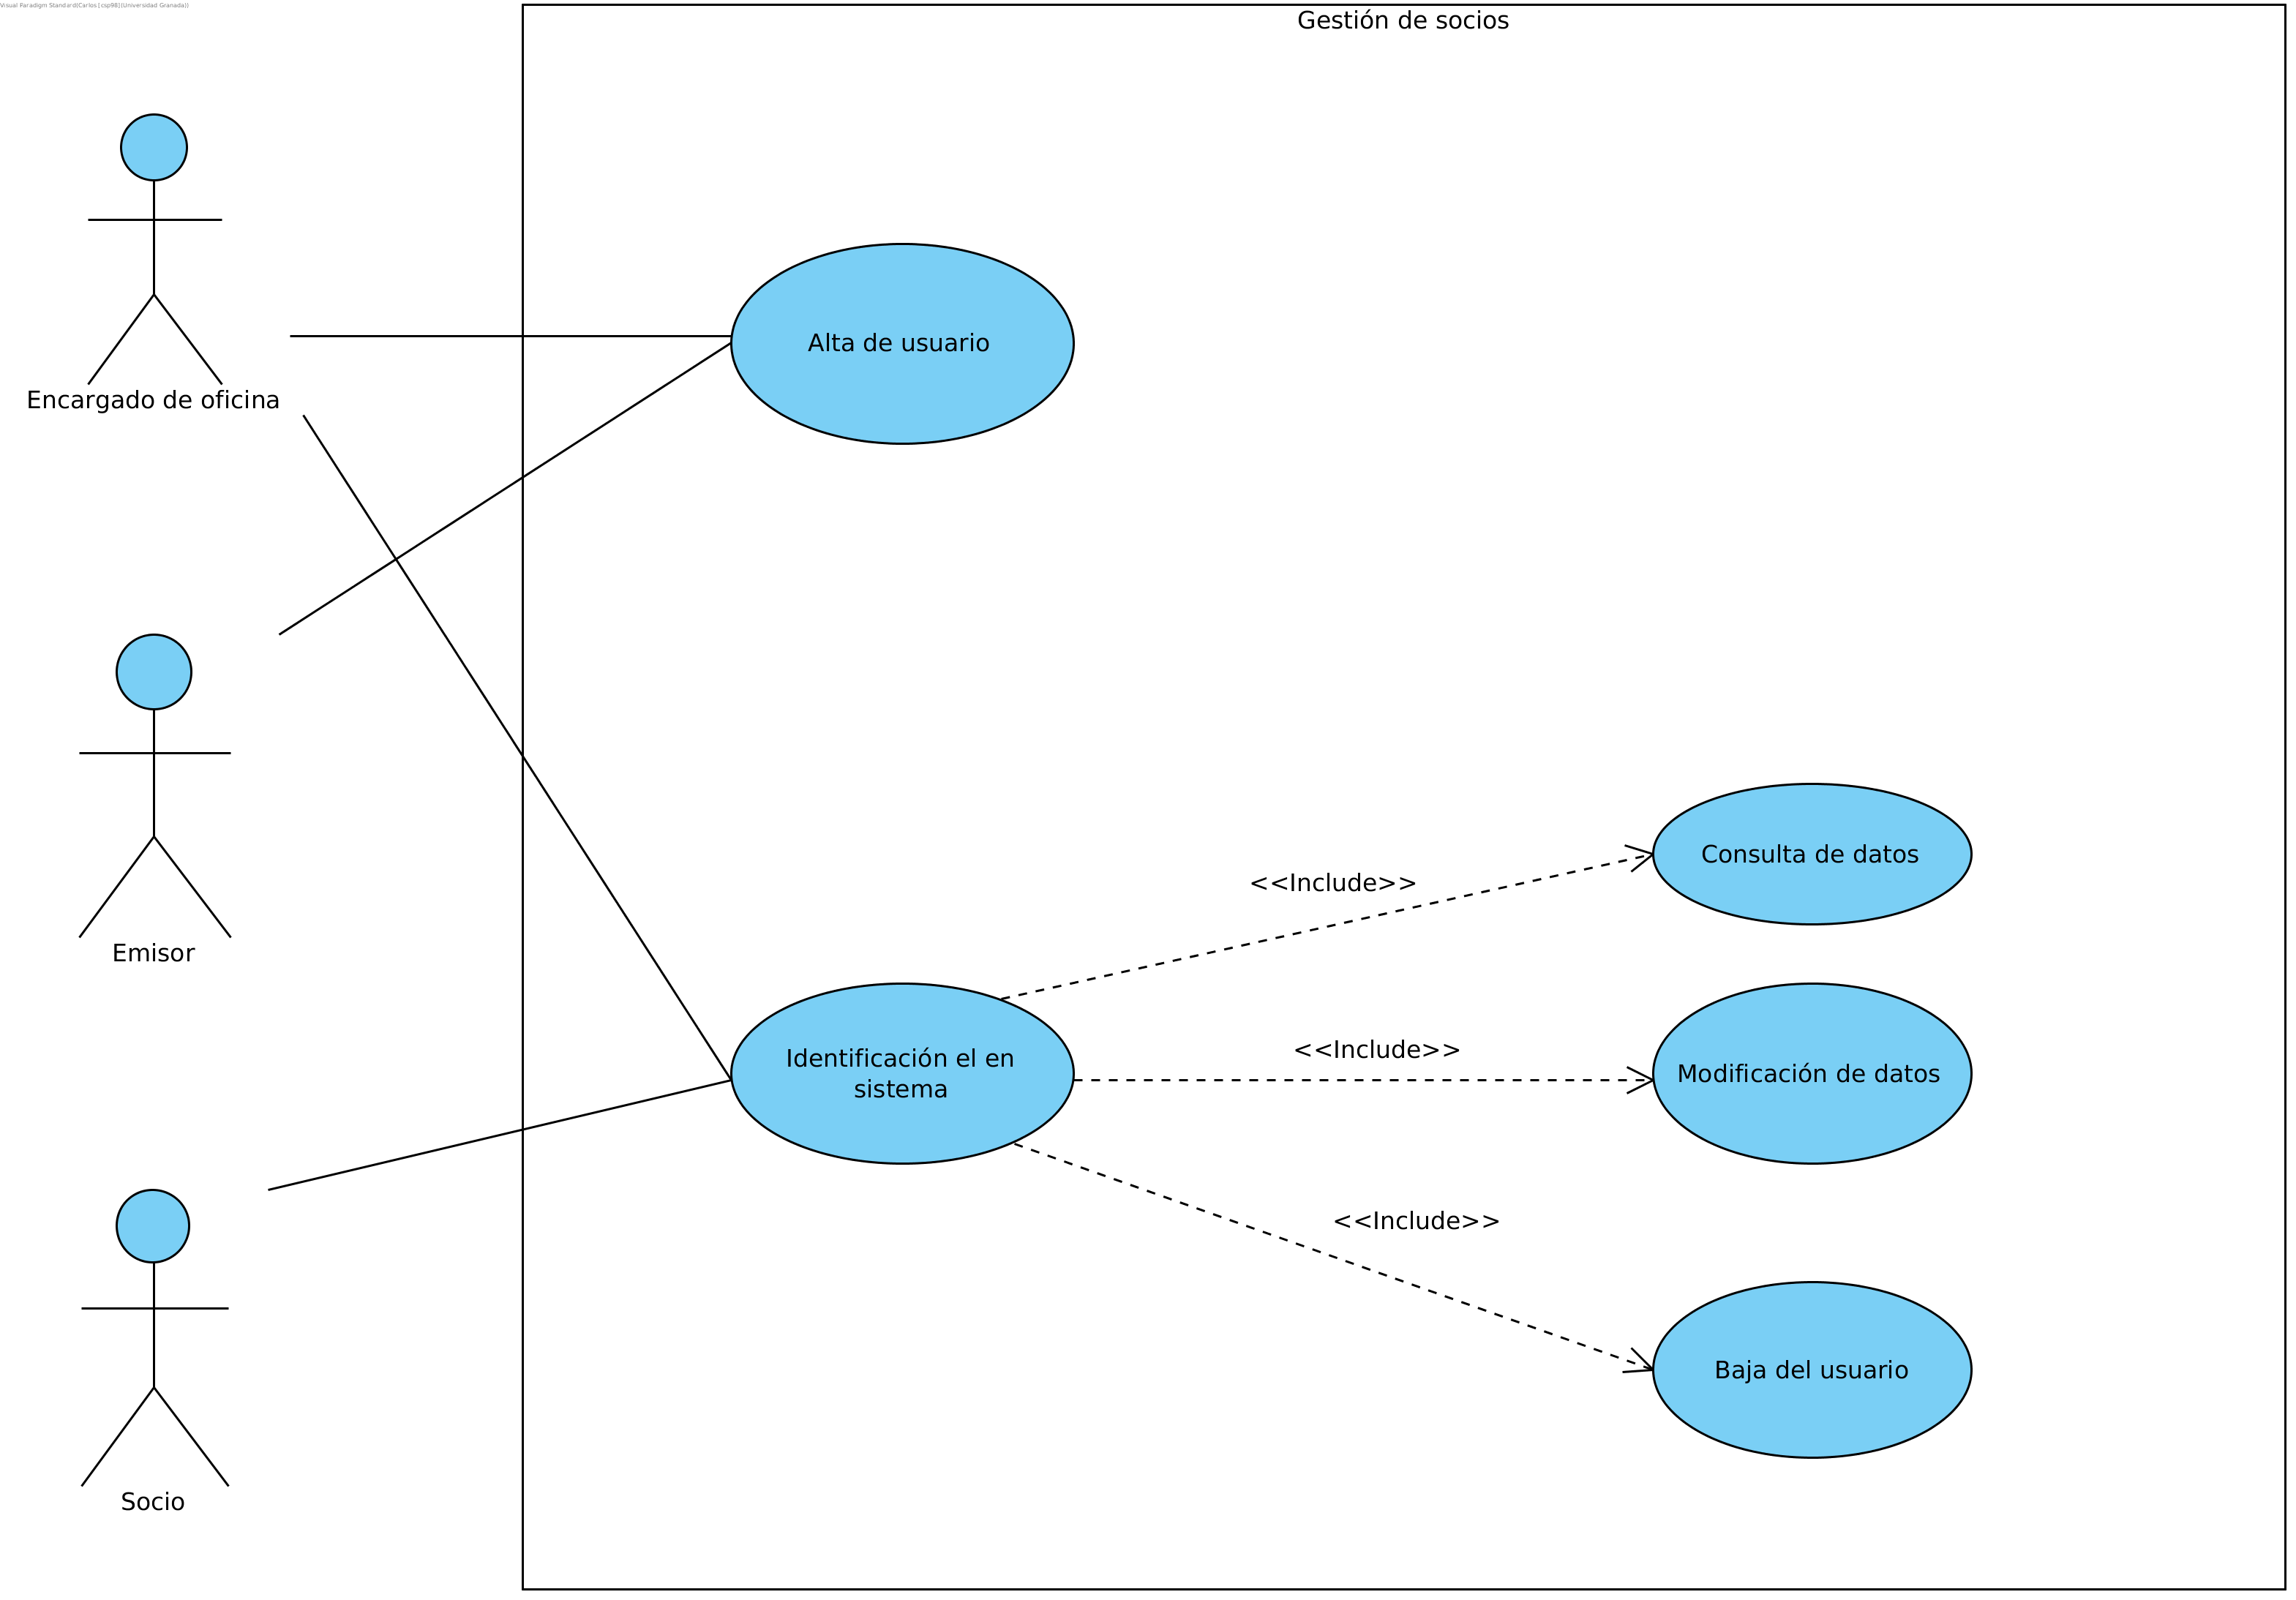
\includegraphics[scale=0.5]{gestion_socios.png}
\caption{Gestionar socios}
\end{figure}

\section{Diagrama de paquetes}

\begin{figure}[H]
\centering
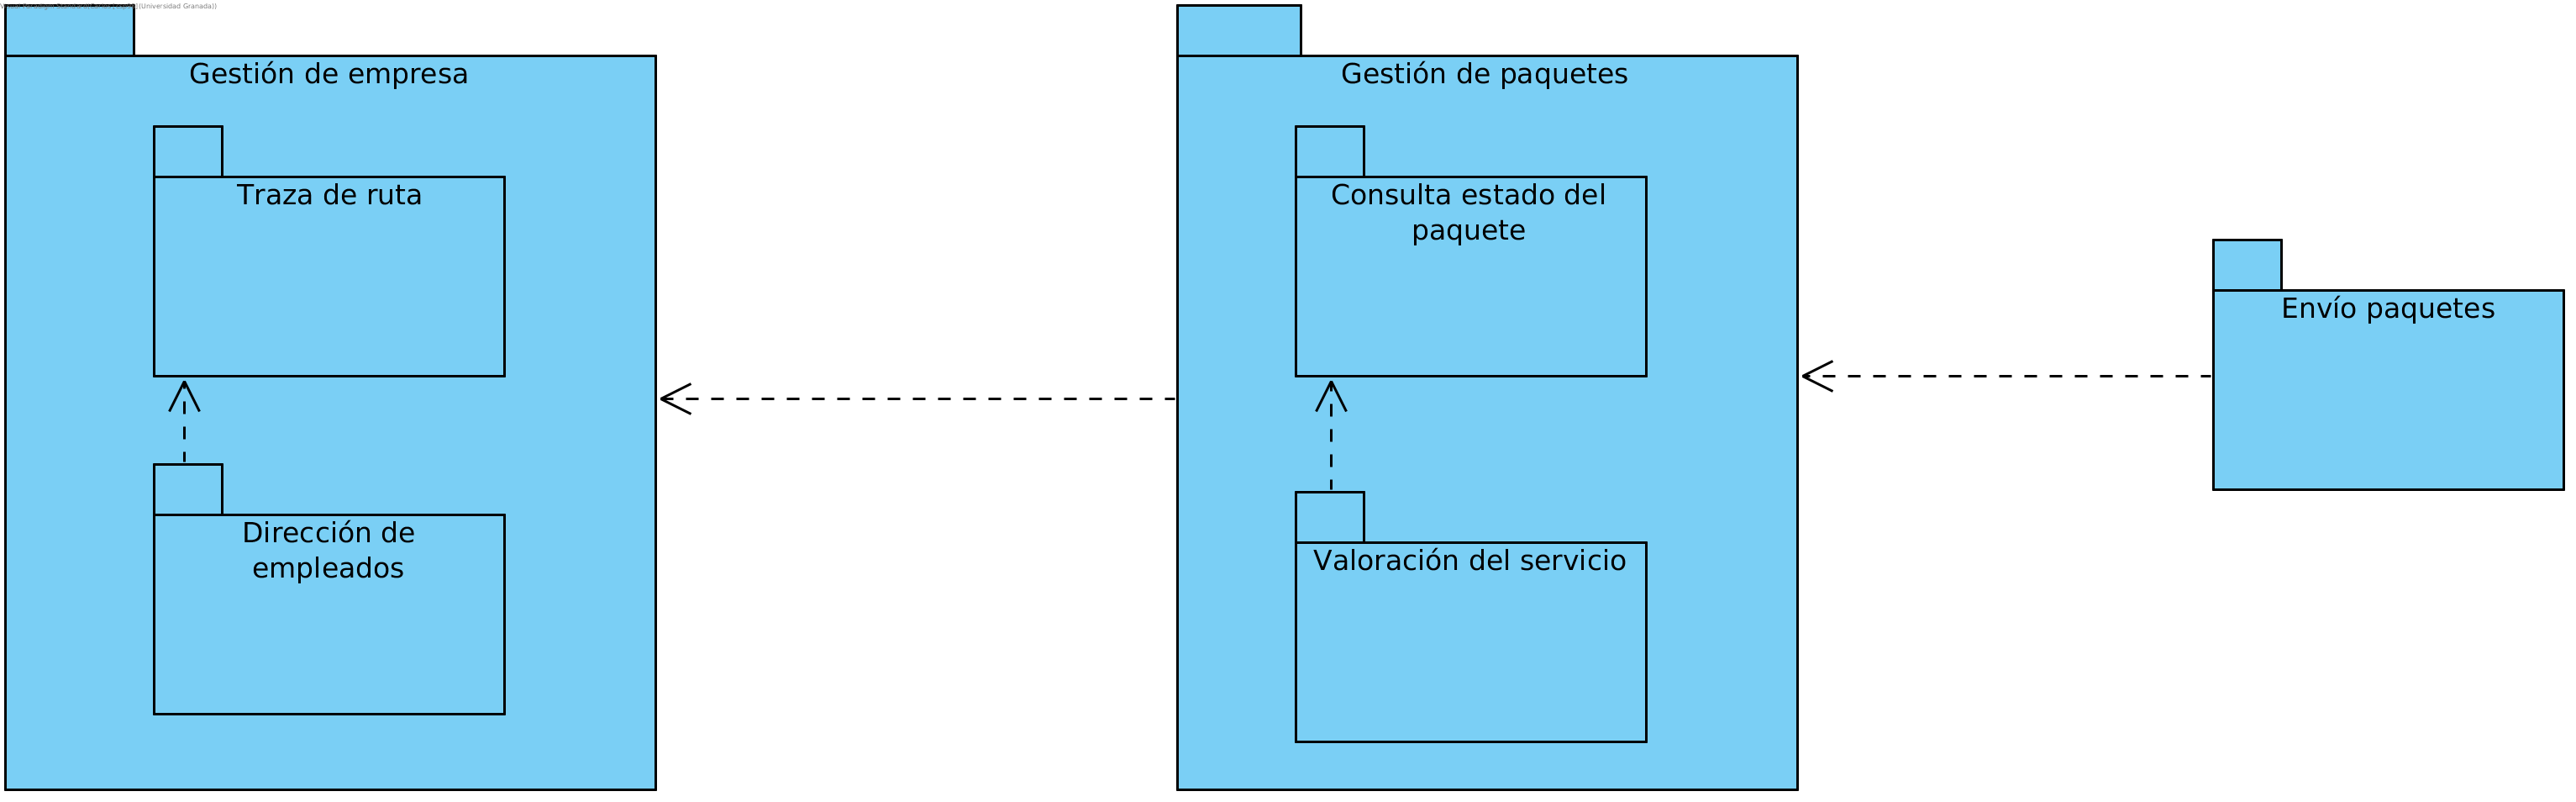
\includegraphics[scale=0.5]{paquetes.png}
\caption{Diagrama de paquetes}
\end{figure}

\section{Descripción de casos de uso a nivel general}

\subsection{José Miguel Pelegrina Pelegrina}

\subsection{José Baena Cobos}

\subsection{Carlos Sánchez Páez}


%%%%%%%%%%%%%%%%%%%%%%%%%%%%Fin del documento%%%%%%%%%%%%%%%%%%%%%%%%%%%%%%%%%
\end{document}
